\documentclass[a4paper,14pt]{extreport}
\usepackage[left=1.5cm,right=1.5cm,
    top=1.5cm,bottom=2cm,bindingoffset=0cm]{geometry}
\usepackage{scrextend}
\usepackage[T1,T2A]{fontenc}
\usepackage[utf8]{inputenc}
\usepackage[english,russian,ukrainian]{babel}
\usepackage{tabularx}
\usepackage{amssymb}
\usepackage{color}
\usepackage{amsmath}
\usepackage{mathrsfs}
\usepackage{listings}
\usepackage{graphicx}
\graphicspath{ {./images/} }
\usepackage{lipsum}
\usepackage{xcolor}
\usepackage{hyperref}
\usepackage{tcolorbox}
\usepackage{tikz}
\usepackage[framemethod=TikZ]{mdframed}
\usepackage{wrapfig,boxedminipage,lipsum}
\mdfdefinestyle{MyFrame}{%
linecolor=blue,outerlinewidth=2pt,roundcorner=20pt,innertopmargin=\baselineskip,innerbottommargin=\baselineskip,innerrightmargin=20pt,innerleftmargin=20pt,backgroundcolor=gray!50!white}
 \usepackage{csvsimple}
 \usepackage{supertabular}
\usepackage{pdflscape}
\usepackage{fancyvrb}
%\usepackage{comment}
\definecolor{ggreen}{rgb}{0.4,1,0}
\definecolor{rred}{rgb}{1,0.1,0.1}
\usepackage{array,tabularx}
\usepackage{colortbl}

\usepackage{varwidth}
\tcbuselibrary{skins}
\usepackage{fancybox}


\usepackage[framemethod=TikZ]{mdframed}
\usetikzlibrary{calc}
\makeatletter
\newlength{\mylength}
\xdef\CircleFactor{1.1}
\setlength\mylength{\dimexpr\f@size pt}
\newsavebox{\mybox}
\newcommand*\circled[2][draw=blue]{\savebox\mybox{\vbox{\vphantom{WL1/}#1}}\setlength\mylength{\dimexpr\CircleFactor\dimexpr\ht\mybox+\dp\mybox\relax\relax}\tikzset{mystyle/.style={circle,#1,minimum height={\mylength}}}
\tikz[baseline=(char.base)]
\node[mystyle] (char) {#2};}
\makeatother

\definecolor{amber}{rgb}{1.0, 0.75, 0.0}
\definecolor{babyblue}{rgb}{0.54, 0.81, 0.94}

\usepackage{float}
\usepackage{wrapfig}
\usepackage{framed}
%for nice Code{
\lstdefinestyle{customc}{
  belowcaptionskip=1\baselineskip,
  breaklines=true,
  frame=L,
  xleftmargin=\parindent,
  language=C,
  showstringspaces=false,
  basicstyle=\small\ttfamily,
  keywordstyle=\bfseries\color{green!40!black},
  commentstyle=\itshape\color{purple!40!black},
  identifierstyle=\color{blue},
  stringstyle=\color{orange},
}
\lstset{escapechar=@,style=customc}
%}


\begin{document}
\pagecolor{white}

%----------------------------------------1
\newtcbox{\xmybox}[1][red]{on line,arc=7pt,colback=#1!10!white, colframe=#1!50!black, before upper={\rule[-3pt]{0pt}{10pt}},boxrule=1pt, boxsep=0pt,left=6pt,right=6pt,top=2pt,bottom=2pt}

\begin{center}\xmybox[amber]{Мнацаканов Антон Станіславович} \xmybox[amber]{ДП-82} \xmybox[amber]{Варіант №5} \end{center}


\begin{center}\xmybox[red]{Пароварка}\end{center}
Пристрій для приготування їжі на парі. Обраний мною пристрій має конструкцію каструлі з перфорованою вкладкою або ґратами для приготування.

\begin{figure}[h]
\center{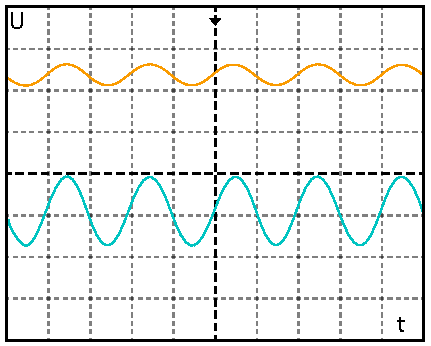
\includegraphics[width=1\linewidth]{12.pdf}}
\caption{Склад системи}
\label{ris1}
\end{figure}

\begin{figure}[h]
\center{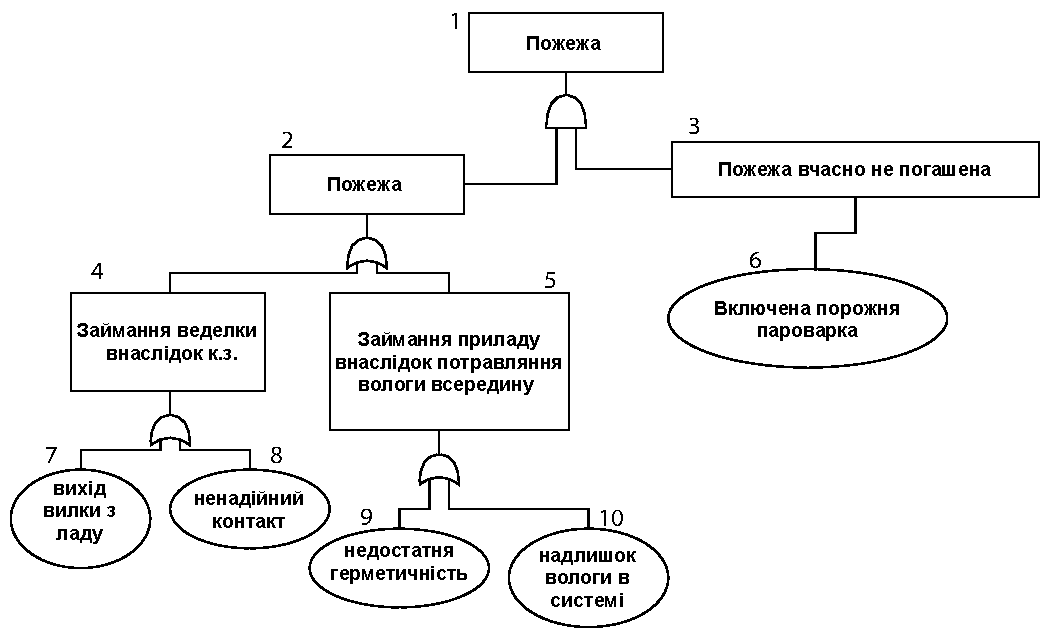
\includegraphics[width=1\linewidth]{1.pdf}}
\caption{Дерево відмов для небезпечної події "пожежа" (при використанні пароварки)}
\label{ris2}
\end{figure}
\newpage
Вираз для визначення ймовірності головної події:\\
\begin{align}
  \begin{cases}
    P_1 = P_2 x P_3\\
    P_2 = 1-(1-P_4)x(1-P_5)\\
    P_3 = P_6\\
    P_4 = 1-(1-P_7)x(1-P_8)\\
    P_5 = 1-(1-P_9)x(1-P_10)
  \end{cases}
\end{align}

\begin{center}$\Downarrow$\\
\vspace{0.4cm}

$P_1 = 1-((1-P_7) x (1-P_8)) x ((1-P_9) x (1-P_10)) x P_6$
\end{center}

\textbf{Висновок}: завжди треба звертати особливу увагу на застереження по експлуатації приладу, а особливо на найголовніші (в моєму випадку): нівякому разі неможна опускати нижній відсік пароварки в воду або промивати під струменем води (в разі подальшого використання це може призвести до короткого замикання або ураження срумом), перед підключенням приладу необхідно переконатись, що вказана на ньому номінальна напруга відповідає напрузі у мережі та використовуйте даний пристрій тільки по його призначенню, як описано в інструкції.

\end{document}
